\chapter{Implementación}
\label{ch:chap04}

El siguiente capítulo encapsula los detalles de implementación y optimización de los algoritmos que se han desarrollado con el objetivo de computar los factores de forma simples y extendidos.

\section{Cálculo de factores de forma de la componente difusa}
\label{sec:dif-impl}

\subsection{Algoritmo del hemi-cubo}

El algoritmo del hemi-cubo fue implementado utilizando la API OpenGL que provee de interfaces de alto nivel para la programación de tarjetas gráficas que facilitan el uso de algoritmos como el del Z-Buffer además de facilitar el manejo de memoria en la GPU.

Para implementar el cálculo de factores de forma se implementará la función \verb|computeFormFactors| como se aprecia en la figura \ref{img:procesado}. Recordando la arquitectura diseñada, la función debe computar completamente la matriz de factores de forma. Esta función seguirá un conjunto de etapas:

\begin{enumerate}
	\item En primera instancia, se configurarán los \textit{buffers} de memoria necesarios para representar el hemi-cubo que se dibujará.
	Para ello, se crea un \textit{Frame Buffer Object} en la GPU que estará compuesto de 5 texturas, cada una de ellas correspondiente a una de las caras a dibujar. Cabe destacar, que estas texturas se compondrán de dos imágenes, una de ellas contiene enteros sin signo que serán utilizados para representar un \verb|id| de cara parche de la escena y la restante contiene los valores de profundidad necesarios para el algoritmo del Z-Buffer.
	\item En la segunda se establecen las matrices de transformación de vista, es decir, las transformaciones lineales que alinean el volúmen de vista al hemicubo. Esto implica trasladar el origen de vista a el baricentro de la cara en cuestión, y alinearla a su normal como se ve en la figura.
	\item En la tercer etapa se procede a dibujar cada objeto en la escena desde el parche considerado en las cinco texturas que componen el hemi-cubo. Con el objetivo de tener el mejor rendimiento posible, se hace uso de los \textit{geometry shaders} para realizar una única llamada de dibujado por objeto. Este método solamente realiza un cambio de \textit{render target}, una de las operaciones más costosas según \ref{img:statechangescost}. Como puede apreciarse en \ref{alg:renderHemicube} solo se realiza una única llamada de \textit{binding} del hemi-cubo. Específicamente, la implementación sigue el siguiente patrón:
	\begin{enumerate}
		\item El \textit{vertex shader} es simplemente \textit{passthough} lo que signfica que conecta las entradas proveídas por la CPU con su salida.
		\item El \textit{geometry shader} genera cinco primitivas donde cada una estará en las coordenadas correspondientes a los frustums de las caras del hemicubo además de añadir un plano adicional de corte del dibujo necesario debido a la imposibilidad de que las caras laterales posean una resolución menor a la cara superior.
		\item El \textit{fragment shader} corregirá el identificador local \verb|gl_PrimitiveId| a un identificador global a partir de variables uniformes que conservan el valor de caras cúbicas y triangulares que componen el objeto. Luego, escribirá el identificador de la cara detectada en la textura que le corresponda según el valor asignado por el \textit{geometry shader}.
	\end{enumerate}
	\item En última instancia es necesario procesar la información del hemi-cubo dibujado para obtener una nueva fila de la matriz $\mathbf{F}$. Este proceso puede ser realizado tanto en GPU como CPU y sigue el patrón visto en \ref{alg:processHemicube}. Ambos métodos fueron implementados y se detallan a continuación:
	\begin{itemize}
		\item Reducción en GPU: Se utilizan \textit{compute shaders} para reducir las cinco texturas que componen el hemi-cubo en un único \textit{Shader Buffer Object} que representa un arreglo de bytes en la GPU. En este caso, el arreglo representará una fila completa de la matriz. Para calcular cada entrada se utiliza una textura inmutable auxiliar que contiene los valores de corrección propuestos por \citeauthor{Cohen} en conjunción con la función \verb|atomicAdd| para sumar las componentes de los factores de forma de cada elemento. Es necesario que esta operación sea atómica para garantizar que dos procesadores no escriban en la misma posición del arreglo de forma concurrente.
		Este arreglo accesible desde la CPU ediante la función \verb|glMapBuffer|, que a través del dispositivo DMA (del inglés \textit{Direct Memory Access}) permite la lectura de la memoria VRAM de forma directa aunque requiere de la sincronización entre GPU-CPU.
		No obstante, dada la naturaleza de las tarjetas gráficas la adición de condicionales hace que las instrucciones SIMD generen divergencia de hilos y por tanto reducen drásticamente el rendimiento del algoritmo.
		\item Reducción en CPU: Con el objetivo de aumentar el rendimiento del algoritmo se utiliza la reducción en CPU, en este caso, se utiliza la función \verb|glReadPixels| que sincroniza la GPU y copia el contenido de la memoria VRAM en la memoria RAM. Luego, se inician hilos de CPU que procesan a información de manera similar a la GPU, aunque de forma secuencial para eliminar la necesidad de barreras de sincronización,  mientras tanto se sigue procesando nuevos hemi-cubos en la GPU generando un máximo de concurrencia entre los dispositivos.
	\end{itemize}
 \end{enumerate}

\begin{algorithm}
	\caption{Algoritmo de proyección de la escena en un hemi-cubo}
	\label{alg:renderHemicube}	
	\begin{algorithmic}
		\Function{$computeFormFactors$}{}
		\State $bindHemicube()$
		\Loop{$face \in scene$}
		\State $alignCamera(face)$
		\State $clearBuffers()$
		\State $render(scene)$
		\State $hemicube \gets getHemicube()$
		\State $startThread(processHemicube, face, hemicube)$
		\EndLoop
		\EndFunction
	\end{algorithmic}
\end{algorithm}

\begin{algorithm}
\caption{Procesamiento de una fila de la matriz $\mathbf{F}$ a partir de la información almacenada en una textura cúbica.}
\label{alg:processHemicube}
\begin{algorithmic}
		\Function{$processHemicube$}{$face, hemicube$}
			\State $row \gets [0,...,0]$
			\Loop{$\text{ }pixel \in hemicube:$}
				\State $factor \gets getCorrectionFactor(pixel)$
				\State $seenFace \gets getFaceId(pixel)$
				\If{$isValid(seenFace)$}
					\State $row[seenFace] \gets + factor$
				\EndIf
			\EndLoop
			\State $formFactorMatrix[face] \gets  row$
		\EndFunction
\end{algorithmic}
\end{algorithm}

\vspace{5mm}
\begin{minipage}[h]{\linewidth}
	\centering
	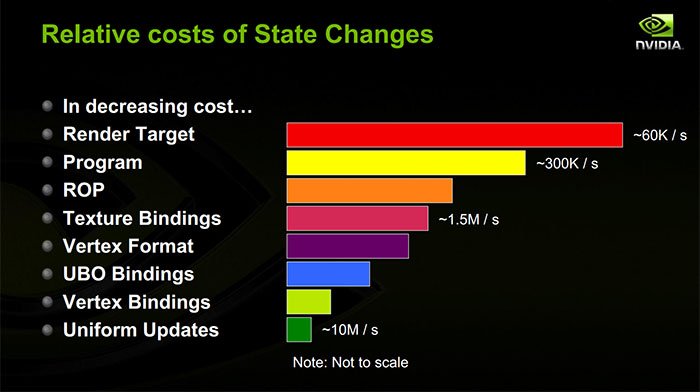
\includegraphics[width=\linewidth]{assets/statecosts}
	\captionof{figure}{Costo de cambios de estado en OpenGL. Fuente: Nvidia}
	\label{img:statechangescost}
\end{minipage}

\subsection{El algoritmo de la hemi-esfera}
El algoritmo de la hemi-esfera fue implementado utilizando la biblioteca de traza de rayos Embree. Esta biblioteca soporta el trazado de rayos en la CPU en múltiples superficies, en particular, triángulos y cuadriláteros utilizando BHV (del inglés \textit{Bounding Volume Hirarchies}). Estas estructuras de datos se basan en árboles que sub-dividen la escena en un conjunto de volúmenes simples que encapsulan un grupo de primitivas geométricas, cada nivel garantiza la reducción de tamaño de dichas estructuras. Su utilidad radica en la simplificación del cálculo de la intersección rayo-objeto, pues esta la computación de la intersección de un rayo con un volumen envolvente tiene un costo de cómputo despreciable en comparación al muestreo en una gran cantidad de primitivas. La aceleración proviene en caso de fallo, pues un fallo en la intersección del rayo con el volumen envolvente supone a su vez el fallo de la intersección con todos las primitivas que contiene.

\begin{algorithm}
	\caption{Cálculo de una fila de los factores de forma utilizando traza de rayos}
	\label{alg:processHemicube}
	\begin{algorithmic}
		\Function{$computeFormFactors$}{$face$}
			\State $row \gets [0,...,0]$
			\State $directions \gets beckers(nSamples)$
			\State $baricenter \gets face.getBaricenter()$
			\Loop{$\textbf{ in parellel }direction \in directons:$}
			\State $intersection \gets traceRay(scene, baricenter, directions)$
			\State $seenFace \gets getFaceId(intersection)$
			\If{$isValid(seenFace)$}
			\State $row[seenFace] \gets + \frac{1}{nSamples}$
			\EndIf
			\EndLoop
			\State $formFactorMatrix[face] \gets  row$
		\EndFunction
	\end{algorithmic}
\end{algorithm}

De forma similar a \ref{sec:hemicubehgl} es necesario posicionar el origen de cada rayo a trazar en el baricentro de la superficie. Luego, recordando \eqref{ffhemiesfera}, es necesario generar un conjunto de direcciones utilizando la distribución del coseno o similar. Si bien originalmente se utilizó la generación de números pseudo-aleatorios para generar rayos correctamente distribuidos, el uso de números aleatorios perjudicó el rendimiento del algoritmo dada la complejidad de los algoritmos que lo computan. Es por esto que se decidió utilizar otro algoritmo de generación de direcciones determinísticas en una hemi-esfera, en este caso la \textit{regla general de particionado de una hemi-esfera en celdas de área equitativa} propuesta por \citeauthor{Becker}. Estas direcciones son pre-calculadas y almacenadas pues previo al procesamiento de se conoce la definición (o cantidad de rayos) que se utilizarán en el cálculo.

Luego se procede a la traza de rayos, $\mathbf{F}_{ij}$ se calculará como $\frac{nIntersecciones_{ij}}{nMuestras}$, esto significa que por cada rayo que parta de la superficie $S_{i}$ impactando $S_{j}$ se adiciona $\frac{1}{nMuestras}$ al valor de la entrada correspondiente en $\mathbf{F}$.

El muestreo de puntos partiendo del origen de la hemi-esfera en las direcciones determinadas se calcula utilizando la función \verb|rtcIntersect1|, que retorna, de forma similar a OpenGL un identificador de primitiva relativo al objeto que se dibuja. Para transformarlo en un identificador global se utilizan los valores obtenidos \verb|geomID| y \verb|primID| además de un mapa de \textit{offsets} que contienen un número con la cantidad de primitivas que anteceden a un objeto. Obtenido el conjunto de primitivas vistas, resta reducirla para generar una fila de la matriz adicionando $\frac{1}{nMuestras}$ para cada rayo.

\section{Cálculo de factores de forma de la componente especular}

El cálculo de factores de forma extendido en fue implementado en dos variantes para el método del hemi-cubo, y de una única manera para el algoritmo de trazado de rayos.

\subsection{Extensión del método del hemi-cubo}
Ambas variantes son métodos de "dos pasadas", es decir, se dibujará el hemicubo normalmente y luego de determinar cuales de las caras visibles son reflectivas se proyectará nuevamente la escena para determinar qué parches son visibles debido al fenómeno de reflexión.

Los métodos utilizados son heurísticos y su factor de error depende drásticamente del área de los parches, ya que al contrario de la técnica de trazado de rayos se desconoce el punto exacto en que los rayos emitidos desde el hemicubo colisionan con los parches del entorno.

La primer variante utiliza el método de dibujado de portales en la GPU, mientras que la segunda fue implementada utilizando \textit{trazado de rayos} en la CPU.

\subsubsection{Dibujado de portales}

El dibujado de portales es una técnica que emplea la rasterización para recortar el \textit{frame buffer} en los puntos cubiertos por cierta superficie ubicada en el entrorno tri-dimensional (como una ventana o una puerta). Normalmente se utiliza esta técnica para optimizar el dibujado de escenas donde la oclusión entre objetos es alta o en la simulación de espejos planos.

Este método puede ser realizado de forma sencilla utilizando la GPU debido a los \verb|Stencil Buffers|, que son similares a los \textit{buffers} de profundidad, pero almacenan información arbitraria que puede ser utilizada para decidir qué \textit{fragmentos} pasan la prueba del \verb|Stencil Test|.

En el caso de la implementación propuesta, el primer paso consiste en dibujar un \textit{stencil buffer} donde se encuentre el parche cuyo coeficiente de reflexión especular es mayor a cero desde la dirección simétrica como se aprecia en \ref{img:espejo}, solo se dibujará la sección del espejo  Luego, manteniendo el mismo volumen de vista, se dibujarán los identificadores de los parches de forma similar al dibujado del hemi-cubo salvo que en una textura bi-dimensional, es necesario además establecer un plano de corte en la superficie especular para evitar el dibujado de los objetos que se encuentren detrás de esta. Este proceso se realiza a una resolución muy baja con el objetivo de preservar el rendimiento y minimizar el costo de transferencia de memoria.

\begin{figure}[H]
	\centering
	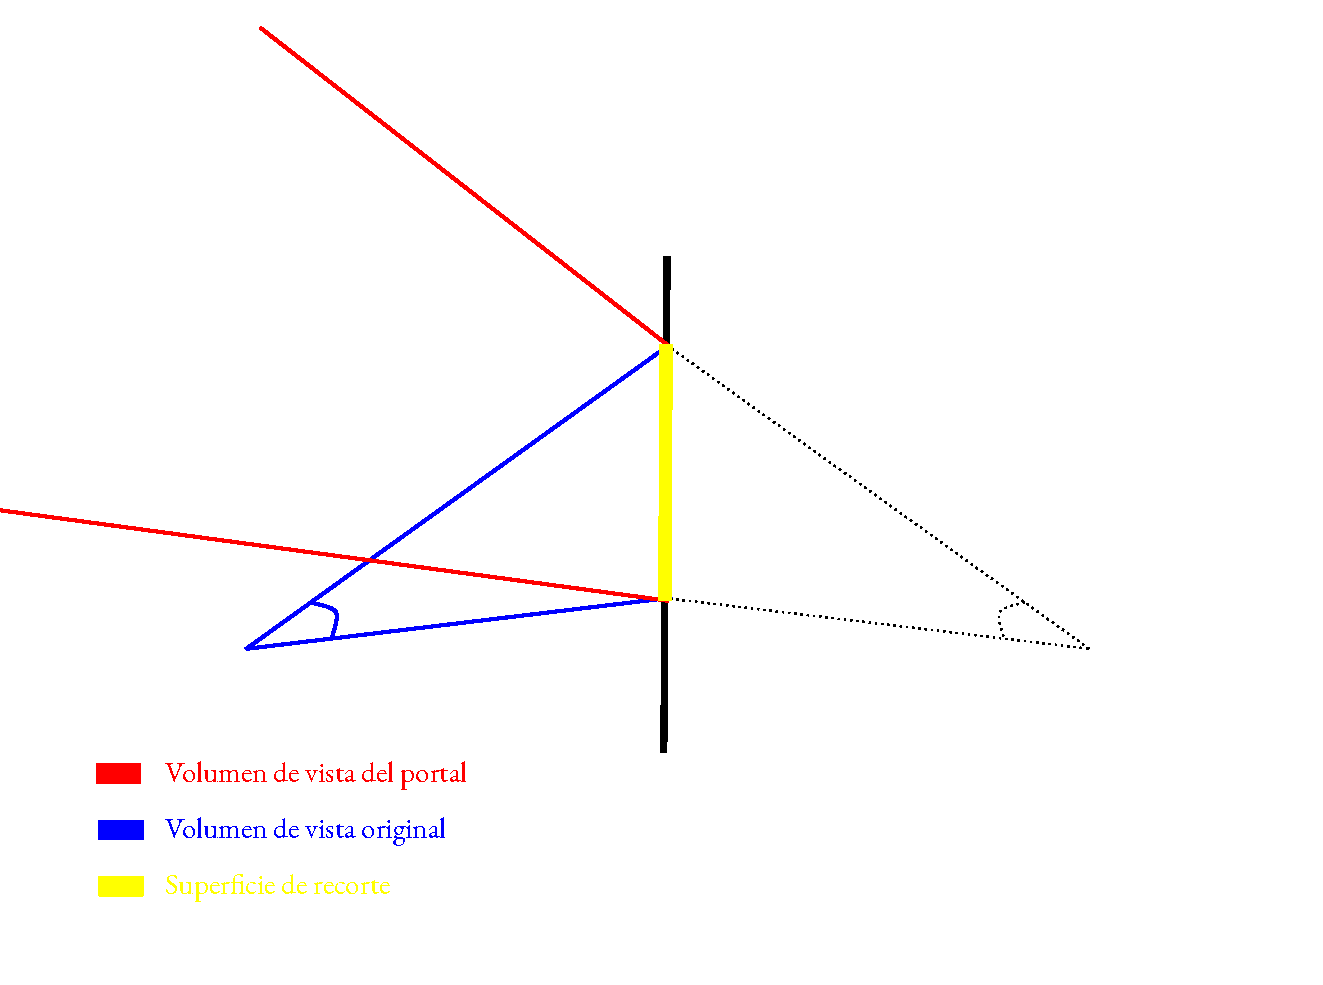
\includegraphics[width=.8\linewidth]{assets/Espejo}
	\captionof{figure}{Generación del volumen de vista para espejos}
	\label{img:espejo}
\end{figure}

Finalmente, se obtienen los identificadores de las caras reflejadas. En caso de que existan caras con valores de reflexión especular no nulos se vuelven a procesar, en otro caso se utilizarán los identificadores obtenidos para distribuir el factor de forma correspondiente al fragmento del hemi-cubo entre los parches visualizados.

\begin{algorithm}
	\caption{Cálculo de las caras vistas utilizando dibujado de portales}
	\label{alg:processHemicube}
	\begin{algorithmic}
		\Function{$renderPortal$}{$face, targetFace$}
		\State $origin \gets face.getBarycenter()$
		\State $direction \gets face.getNormal()$
		\State $setCamera(origin, direction)$
		\State $bindVertices(targetFace)$
		\State $renderStencil(0xFF)$
		\State $refDir \gets reflected(dir, targetFace.getNormal())$
		\State $refOrig \gets symmetrical(origin, targetFace.getPlane())$
		\State $setCamera(refOrig, refDir)$
		\State $bindVertices(scene)$
		\State $setStencilFunction(== 0xFF)$
		\State $render()$
		\State $seenFaces \gets readBuffer()$
		\Loop{$faceId \in seenFaces$}
			\If{$isValid(faceId)$}
				\State $row[faceId] \gets +(\frac{1}{nSamples})$
				\If{$isReflective(faceId)$}
					\State $renderPortal(targetFace, faceId)$
				\EndIf
			\EndIf
		\EndLoop
		\EndFunction
	\end{algorithmic}
\end{algorithm}

\subsubsection{Método híbrido}

El método híbrido consiste en la utilización del trazado de rayos para computar qué parches son visualizados desde el parche considerado. Para ello, se trazarán rayos desde un conjunto de puntos pertenecientes al parche reflectivo de manera uniformemente distribuida, la dirección es la que corresponde a la del voluen de vista, es decir, la que está dada por la diferencia entre los baricentros del parche de origen y del especular. Las caras vistas, de ser difusas, son las que aportarán fracciones de valor al factor de forma.

Esto emula el fenómeno de la reflexión, aunque introduce pequeños errores al aproximar la dirección real de reflexión (aquella dada por la diferencia entre el baricentro del parche considerado y el punto de intersección con el rayo).

\begin{figure}[H]
	\centering
	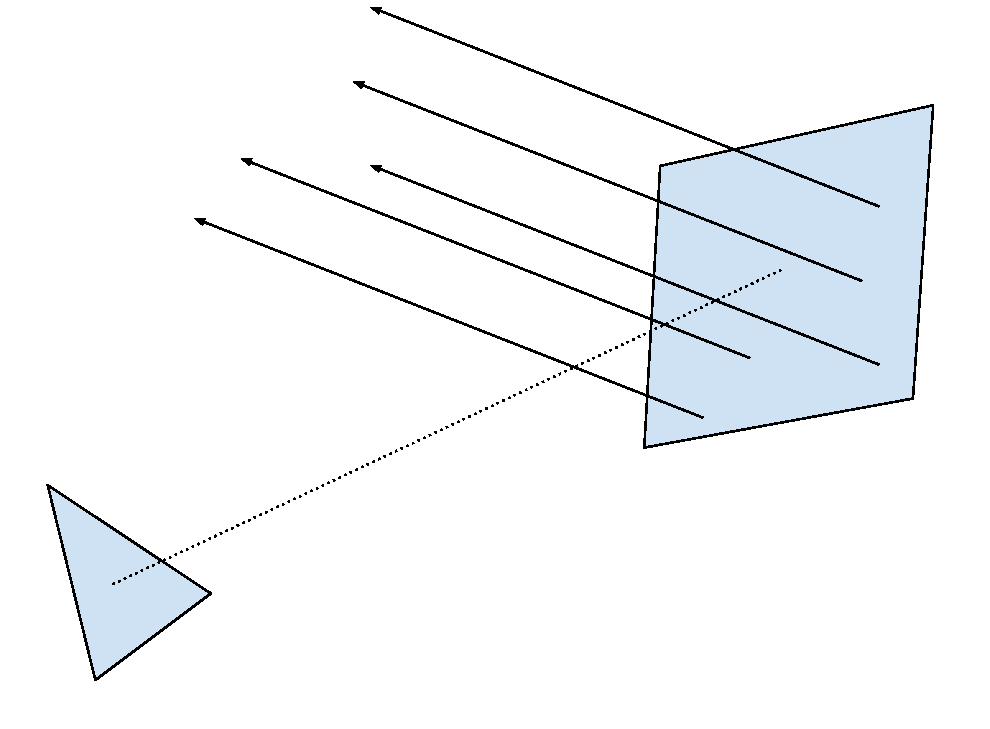
\includegraphics[width=.8\linewidth]{assets/Hibrido}
	\captionof{figure}{Visualización del rebote de rayos al impactar en parches especulares}
	\label{img:hibrido}
\end{figure}

\begin{algorithm}
	\caption{Cálculo de las caras vistas utilizando trazado de rayos}
	\label{alg:processHemicube}
	\begin{algorithmic}
		\Function{$renderReflections$}{$face, targetFace$}
			\State $direction \gets normalize(targetFacegetNormal() - face.getNormal())$
			\State $refDir \gets reflected(dir, targetFace.getNormal())$
			\State $origins \gets getUniformSamples(targetFace)$
			\Loop{$\textbf{ in parallel }origin \in origins$}
				\State $hit \gets traceRay(origin, refDir)$
				\If{$isValid(hit)$}
				\State $row[face] \gets +(\frac{1}{nSamples})$
					\If{$isReflective(faceId)$}
						\State $renderReflections(targetFace, faceId)$
					\EndIf
				\EndIf
			\EndLoop
		\EndFunction
	\end{algorithmic}
\end{algorithm}

\subsection{Extensión del método de la hemi-esfera}

En el caso del trazado de rayos, la extensión de los factores de forma es prácticamente trivial. Comprende la extensión de la función \verb|traceRay()|, que en lugar de retornar un único valor para la cara vista, retornará un conjunto de pares de identificadores de caras y fracción de factor de forma. Básicamente, si el rayo inicial interseca una cara cuyo coeficiente de reflexión especular es estrictamente positivo se almacenará el total de $k(1 - \rho_{j})$ (donde $k = \frac{1}{nMuestras}$) como contribuyente del factor de forma $\mathbf{F}_{ij}$ y se calcularán las siguientes intersecciones con el \textit{residuo} de la reflexión que se distribuirá en los factores de forma que correspondan a la reflexión. Es decir, suponiendo que un rayo impacta $S_{k}$ desde el camino $(S_{i}, S_{j})$ donde $\rho_{j} \ge 0$ se agregará $k\rho_{j}(1 - \rho_{k})$ y se procederá de forma recursiva hasta que $\rho_{z} = 0$ para una superficie intersecada $S_{z}$ o se alcance el máximo límite de recursión cómo se aprecia en la Figura \ref{img:caminoespecular}.

\section{Cálculo del vector de radiosidad}

Recordando \ref{sec:vrad}, se han propuesto dos métodos para resolver el sistema. El método exacto supone hallar el vector solución del sistema de ecuaciones dado por $(\mathbf{I - RF}B) = E$, el segundo método está regido por el método iterativo dado por \eqref{eq:iterativo}.

En el primer caso, la implementación se realizó utilizando la biblioteca de álgebra lineal \textit{Eigen} pues soporta la resolución de sistemas con matrices esparzas. En este caso, dadas las características de la matriz se optó por añadir soporte para los siguientes métodos:

\begin{itemize}
	\item{De factorización}
		\begin{itemize}
			\item{Descomposición LU:} En matrices no singulares (hemos demostrado que $\mathbf{I - RF}$ no lo es), la descomposición $\mathbf{LU}$ genera dos matrices tal que $\mathbf{M} = \mathbf{LU}$ con $\mathbf{L}$ triangular inferior y $\mathbf{U}$ triangular superior. Fácilmente se puede comprobar que  $\mathbf{M}^{-1} = \mathbf{U}^{-1} \mathbf{L}^{-1} \mathbf{I}$. Por tanto, $B =(\mathbf{U}^{-1} \mathbf{L}^{-1} \mathbf{I})E$. 
			\item{Descomposición de Cholesky:} La factorización supone que  $\mathbf{I - RF}$ se puede descomponer como  $\mathbf{LL^{T}}$ donde  $\mathbf{L}$ es triangular inferior. Esta descomposición permite resolver el sistema trivial a través de las ecuaciones $\mathbf{L}B' = E$ y $\mathbf{L^{T}}B = B'$.
			\end{itemize}
	\item{Iterativos}
			\begin{itemize}
			\item Gradiente conjugado:
				Dada una matriz cuadrada y definida positiva (como $\mathbf{I - RF}$) es posible expresar el vector solución del sistema como $\sum_{i=1}^{N} \alpha_{i}p_{i}$ donde $p_{k}$ es un conjunto de vectores ortonormales. El método de cálculo de $\alpha_{k}$ comprende el cálculo de $\frac{p_{k} \cdot E}{||p_{k}||^{2}}$.			\item Gradiente conjugado estabilizado: Este método ofrece mayor velocidad de convergencia que el anterior, es decir, se necesitan menos iteraciones para alcanzar el resultado deseado. 
		\end{itemize}
\end{itemize}

Por otro lado, se implementó el método completamente iterativo dado por \eqref{eq:iterativo}. Este método es similar en precisión a los métodos iterativos  mencionados anteriormente pues no se calcula el valor exacto de $B$. Para su implementación se utilizó la bibliotecta \textit{Eigen} para realizar la multiplicación de matrices esparzas.

Finalmente, luego de calcular el vector de radiosidades se procede a la interpolación y ajuste de resultados. Dado que en OpenGL solo es posible agregar atributos a nivel de vértice y no a nivel de primitiva es necesario generar un vector extendido donde se replica el valor asignado por cara a cada uno de los vértices.

Este proceso puede realizarse de forma trivial, simplemente copiando valores o aplicando interpolación a nivel de geometría como en el modelo de iluminación de \textit{Gouraud}. Este proceso implica balancear el valor de radiosidad para cada vértice asignándole el promedio del valor de radiosidad de cada cara (como se aprecia en \ref{img:interpolation}) en que se encuentre como muestra el algoritmo \ref{alg:inter}.

\begin{algorithm}
	\caption{Algoritmo de interpolación de radiosidad para vértices}
	\label{alg:inter}
	\begin{algorithmic}
		\Function{$interpolate$}{$B$}
			\Loop{$\text{ } vertex \in scene$}
				\State $temp \gets 0$
				\State $faces \gets {face such as vertex \in face}$
				\Loop{$\text{ } face \in faces$}
					\State $temp \gets +B(face)$
				\EndLoop
				\State $vertexRadiosity \gets \frac{temp}{length(faces)}$
			\EndLoop
		\EndFunction
	\end{algorithmic}
\end{algorithm}

\begin{figure}[H]
	\centering
	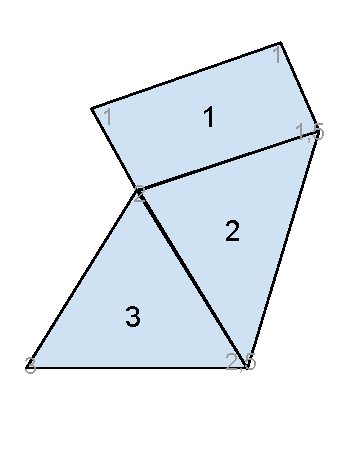
\includegraphics[width=.5\linewidth]{assets/Interpolation}
	\captionof{figure}{Ejemplificación del algoritmo de interpolación}
	\label{img:interpolation}
\end{figure}

Esta técnica genera resultados con figuras de colores menos planas, ocultando la discretización que se realizó para aplicar el método de elementos finitos como se aprecia en la Figura \ref{img:interpolationres}.

\section {Visualización de resultados y resultados intermedios}

La visualización de resultados y resultados intermedios se implementó utilizando el método de \textit{dibujado a textura en capas}. Las texturas en capas son un conjunto de imagenes de igual resolución que contienen distinta información.

El algoritmo implementado no dibuja la escena directamente en el \textit{frame buffer} global de la pantalla. Sin embargo, se dibuja en una textura auxiliar de varios niveles, cada nivel corresponde a una propiedad distinta de la escena. El primer nivel contiene la información del identificador de las caras, el segundo nivel el valor de radiosidad, el tercero el valor de emisión inicial, el ultimo nivel contiene los valores de los coeficientes de reflexión difusa.

Finalmente, para generar la textura que se mostrará en pantalla se utiliza un cuadrilátero unitario. Esta es una técnica estándar para proyectar un valor contenido en un buffer interno en el que corresponde al estándar. Dependiendo de la propiedad que seleccione el usuario, se seleccionará uno de estos niveles para desplegar en pantalla.

Este método, además, añade la posibilidad de implementar la técnica de \textit{picking} que involucra el reconocimiento de la selección que realiza el usuario. Para ello, basta obtener el valor del fragmento (\verb|glReadPixels|) que se encuentra en las coordenadas del puntero dentro de la textura, que son suministradas por el Sistema Operativo.

\section {Interfaz de usuario}

La interfaz de usuario fue implementada utilizando la bibioteca de dibujado de interfaces gráfica en modo inmediato \textit{ImGui}. Este método de dibujado implica que los comandos de dibujado de la interfaz se ejecutan inmediatamente, de forma tal que los resultados son guardados en una máquina de estados. Los componentes dibujados dependen directamente del estado interno de la aplicación, este método era el utilizado en versiones anteriores de OpenGL o Direct3D. Esta biblioteca es reconocida por su capacidad de extenderse a diversas plataformas y por minimizar el impacto en el rendimiento de la aplicación en caso de ser utilizada.